% JointSchemaHead: S + schema -> H (LFM trunk, frozen) -> cross-attn (x2) ->
% decoder (x4, +type embedding) -> gate(lexical prior, MLP) -> softmax.
\begin{figure}[htbp]
\centering
\resizebox{\columnwidth}{!}{%
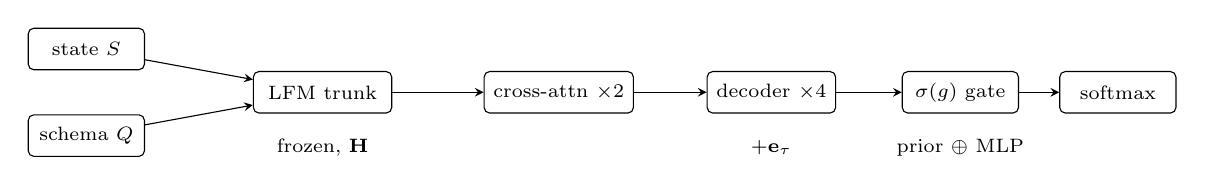
\begin{tikzpicture}[box/.style={draw, rounded corners=2pt, minimum height=1.5em,
  minimum width=4.2em, font=\scriptsize}, arr/.style={->, >=stealth}]
\node[box] (s) at (0,0) {state $S$};
\node[box] (q) at (0,-1.1) {schema $Q$};
\node[box, minimum width=5em] (trunk) at (3, -0.55) {LFM trunk};
\node[box] (xatt) at (6, -0.55) {cross-attn $\times2$};
\node[box] (dec) at (8.7, -0.55) {decoder $\times4$};
\node[box] (gate) at (11.1, -0.55) {$\sigma(g)$ gate};
\node[box] (sm) at (13.1, -0.55) {softmax};
\draw[arr] (s) -- (trunk); \draw[arr] (q) -- (trunk);
\draw[arr] (trunk) -- (xatt); \draw[arr] (xatt) -- (dec);
\draw[arr] (dec) -- (gate); \draw[arr] (gate) -- (sm);
\node[font=\scriptsize] at (3, -1.25) {frozen, $\mathbf{H}$};
\node[font=\scriptsize] at (8.7, -1.25) {$+\mathbf{e}_{\tau}$};
\node[font=\scriptsize] at (11.1, -1.25) {prior $\oplus$ MLP};
\end{tikzpicture}%
}
\caption{JointSchemaHead data flow. Only adapters and head train.}
\label{fig:head}
\end{figure}
